\documentclass{beamer}
\usetheme{Copenhagen}
\usecolortheme{seahorse}

\usepackage{tikz}
\usepackage{graphicx}
\usepackage{listings}
\usepackage{xcolor}
\usepackage{hyperref}
\usepackage{esdiff}

\graphicspath{ {../images/} }

\title{A Random Model of the Primes}
\author{Frank Qiang, Aravinth Venkatesh Natarajan, Anthony Hong}
\institute{Georgia Institute of Technology}
\date{April 25, 2023}

\begin{document}
\frame{\titlepage}
\begin{frame}{Background}
  \begin{itemize}
    \item Infinite number of primes (c. 300 BC, Euclid)
    \item $\pi(x) := \text{number of primes} \leq x$
    \item Prime number theorem: $\pi(x) \sim \frac{x}{\ln x}$ (1896, Hadamard and De la Vall\'ee Poussin)
  \end{itemize}
\end{frame}

\begin{frame}{Prime Gaps}
  \begin{itemize}
    \item Prime gap := difference between a pair of consecutive primes
    \item What does the sequence of prime gaps look like?
      \[[1,2,2,4,2,4,2,4,6,2]\]
      Notice that 1 is the only odd.
    \item How small/large can prime gaps get?
    \begin{itemize}
      \item Small: twin prime conjecture; we have a constant bound by Yitang Zhang (2013), since improved to gap
        $\le 246$ infinitely often
      \item Large: can find gaps of arbitary size (think $n!$); so slightly different goal, want to see how large of a gap we can expect in a given interval
    \end{itemize}
  \end{itemize}
\end{frame}

\begin{frame}{Cramer's Random Model}
  \begin{itemize}
    \item We know prime number distribution isn't exactly random, but it seems to behave that way: try to model as if it were
    \item In the interval $[2, n]$, we expect roughly $\frac{n}{\ln n}$ primes by prime number theorem. There are also roughly $n$ total numbers $[2, n]$. So $n$ has probability $\frac{1}{\ln n}$ of being prime?
    \item Naively assign each $x \in \mathbb{N}_{>2}$ a probability of $\frac{1}{\ln x}$ of being prime
  \end{itemize}
\end{frame}

\begin{frame}{First Iteration}
  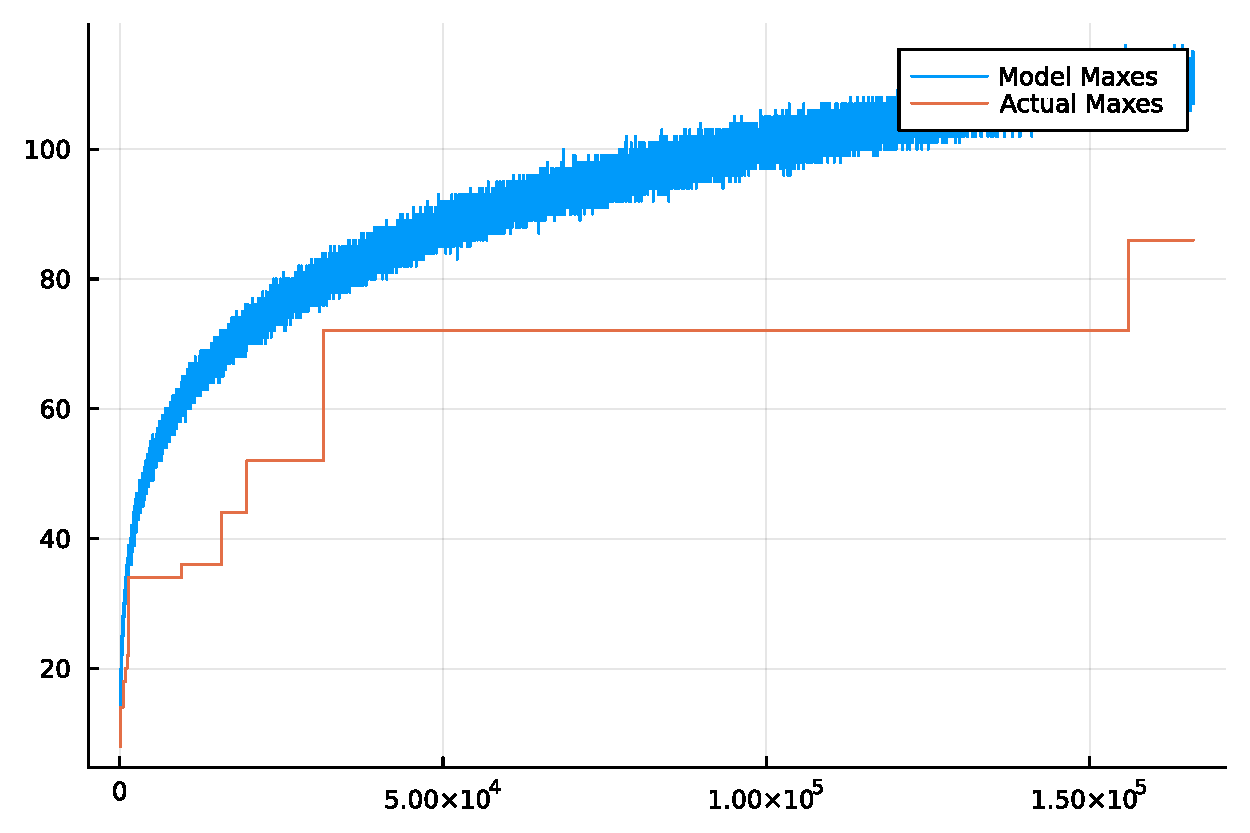
\includegraphics[width=\textwidth]{random-plot1.pdf}

  Plot of estimated largest gap $\le n$ vs. $n$, with
  100 trials per $n$.
\end{frame}

\begin{frame}{Why?}
  \begin{itemize}
    \item We can study this random distribution using ideas from probability and statistics, can give extra insight
    \item Conducting many trials comes at relatively low cost (can be parallelized, will scale with current trend towards multithreaded computers)
    \item We can consider disjoint intervals completely independently (not true of traditional sieve methods)
  \end{itemize}
\end{frame}

\end{document}
